\documentclass[11pt, a4paper]{article}

\usepackage[utf8]{inputenc}
\usepackage{graphicx}
\graphicspath{ {images/} }
\usepackage{mathtools}
\usepackage{amssymb}
\usepackage{amsmath}
\usepackage[english, ngerman]{babel}
\usepackage{cite}
\usepackage{bibgerm}
\usepackage{fullpage}
\usepackage[top=1.5cm,bottom=1.5cm,left=3.5cm,right=2.5cm,headsep=1.5cm,includeheadfoot]{geometry}
\usepackage{tabularx}
\usepackage{eurosym}
\usepackage{enumitem}
\usepackage{multicol}
\usepackage{tikz}
\usepackage{tkz-euclide}
\usepackage{pgfplots}
\usepackage{pdflscape}
\usepackage{acronym}
\usepackage{blindtext}
\usepackage{ifthen}
\usepackage{setspace}
\usepackage{cancel}
\usepackage{color}
\usepackage{listings}
\usepackage{comment}
\usepackage{xcolor}
\usepackage{colortbl}
\usepackage[parfill]{parskip}

\usepackage{fancyhdr}
\pagestyle{fancy}

\fancyhf{} % clear all
\fancyhead[L]{\leftmark}
\fancyfoot[C]{-- \thepage{} --}
%\setlength{\headheight}{15pt}
\renewcommand{\headrulewidth}{0.5pt}
\renewcommand{\footrulewidth}{0pt}
\setlength{\skip\footins}{0.7cm}

\usetikzlibrary{graphs}
\usetikzlibrary{positioning}

\onehalfspacing
\setlength\parindent{0pt}

%\everymath{\displaystyle}

\allowdisplaybreaks

\definecolor{AI-BLUE}{rgb}{0,0.57,0.87}

% Eigene Befehle
\newcommand\q[1]{\glqq{}#1\grqq{}}
\renewcommand\equiv{\Leftrightarrow}
\newcommand\vertequal[2]{\underset{\underset{#2}{\parallel}}{#1}}
\newcommand\cif{\text{if }}
\newcommand\abs[1]{\left|#1\right|}
\newcommand\norm[1]{\abs{\abs{#1}}}
\newcommand\diff[1]{\text{ d#1}}
\newcommand\av[1]{\left\langle#1\right\rangle}
\newcommand\ev[1]{\mathbb{E}\left(#1\right)}
\newcommand\br[1]{\left(#1\right)}
\newcommand\ubr[2]{\underbrace{#1}_{#2}}
\newcommand\quer[1]{\overline{#1}}
\newcommand\setequal{\overset{!}{=}}
\newcommand\dint{\displaystyle \int}
\newcommand\dsum{\displaystyle \sum}
\newcommand\dprod{\displaystyle \prod}
\newcommand\closedInt[2]{\left[#1,#2\right]}
\newcommand{\checkbox}{\Large \Square \normalsize \hspace{0.4cm}}

\newcommand\myref[1]{\ref{#1} (S. \pageref{#1})}
\newcommand\myrefcomma[1]{\ref{#1}, S. \pageref{#1}}

\newcommand\nsm{Nagel-Schreckenberg-Modell }

\begin{document}

\thispagestyle{empty}

\setlength{\hoffset}{-0.5cm} % center title page

\lstset{
  basicstyle=\small,           % the size of the fonts that are used for the code
  breaklines=true,             % sets automatic line breaking
  captionpos=b,                % sets the caption-position to bottom
  frame=single,                % adds a frame around the code
  keepspaces=true,             % keeps spaces in text, useful for keeping indentation of code (possibly needs columns=flexible)
  numbers=right,               % where to put the line-numbers; possible values are (none, left, right)
  showspaces=false,            % show spaces everywhere adding particular underscores; it overrides 'showstringspaces'
  stepnumber=1,                % the step between two line-numbers. If it's 1, each line will be numbered
  tabsize=4,                   % sets default tabsize to 4 spaces
}

\begin{titlepage}
    \begin{center}
    \vphantom{0cm}
    \LARGE \textbf{Dokumentation}\\
    \vspace{3cm}
    \normalsize
    Dokumentation für Simulationstechnik \\
    im Master-Studiengang \textcolor{AI-BLUE}{[Angewandte Informatik]}\\
    an der Ruhr-Universität Bochum\\
    im Wintersemester 2014/15\\
    \vspace{4cm}
    \huge \textbf{Verkehrssimulation mit Zellularautomaten in C++} \\
    \vspace{4cm}
    \normalsize
    \textbf{Projektteilnehmer:}\\
    B. Sc. Christian Andreas Mielers (108 011 204 956)\\
    B. Sc. Phil Yannick Schrör (108 011 214 024)\\
    \vspace{2cm}
    \textbf{Projektbetreuer:}\\
    M. Sc. Markus Scheffer
    \end{center}
\end{titlepage}

\newpage

\pagenumbering{arabic}

\setcounter{page}{2}

\tableofcontents

\newpage


\section{Einleitung}
\label{sec:einleitung}

\newpage
\section{Annahmen}
\label{sec:ansatz}

Im Groben basiert unser Modell auf den Annahmen, die Kai Nagel und Michael Schreckenberg \cite{nagel-schreckenberg} für ihr STCA-Verkehrsmodell (STCA = Standard Zellular-Automat) getroffen haben. Um das Modell jedoch an die Verhältnisse auf deutschen Straßen anzupassen, wurden einige Änderungen vorgenommen.
Im Folgenden werden die unserem Modell zugrunde liegenden Annahmen aufgeführt:\\

\begin{itemize}
\item Es gilt weiterhin, dass eine Zelle 7,5 Meter lang ist und jede Zelle nur ein einziges Fahrzeug zur gleichen Zeit aufnehmen kann.
\item Im klassichen \nsm gibt es die Geschwindigkeitsstufen 0 bis 5. Diese entsprechen Geschwindigkeiten von 0 km/h bis 135 km/h in 27 km/h Abständen. Da uns 135 km/h als Höchstgeschwindigkeit auf einer deutschen Autobahn zu wenig erschienen, haben wir die Höchstgeschwindigkeit auf 7 erhöht, so dass Fahrzeuge nun eine Maximalgeschwindigkeit von 189 km/h erreichen können.
\item Während im \nsm alle Fahrzeuge üblicherweise die gleiche Maximalgeschwindigkeit erreichen können, werden in unserem Modell die Maximalgeschwindigkeiten der Fahrzeuge aus einer Normalverteilung gezogen, deren Mittelwert und Standardabweichung vom Nutzer des Programms frei gewählt werden können. Wir halten dieses Szenario für realistischer, da in der Realität unterschiedliche Fahrzeugtypen unterschiedliche Maximalgeschwindigkeiten erreichen können. Falls vom Nutzer keine Varianz bei den Maximalgeschwindigkeiten gewünscht ist, kann er die Standardabweichung sehr klein wählen, so dass es sehr unwahrscheinlich wird, eine Maximalgeschwindigkeit ungleich dem Mittelwert zu erhalten. Es ist zu beachten, dass es nicht möglich ist, auf diese Weise Fahrzeugen Maximalgeschwindigkeiten zuzuweisen, die 3 unter- oder 7 überschreiten. Dies ist dadurch begründet, dass in Deutschland nur solche Fahrzeuge eine Autobahn befahren dürfen, welche eine Höchstgeschwindigkeit von mindestens 60 km/h erreichen können. Ein Fahrzeug mit der Geschwingkeitsstufe 2 als Höchstgeschwindigkeit (= 54 km/h) würde diesen Grenzwert um 6 km/h unterschreiten.
\item Um das Fahrverhalten unterschiedlicher Fahrertypen abbilden zu können, wird der Trödelfaktor eines jeden Fahrzeugs randomisiert bestimmt. Zu diesem Zweck wird jedoch keine Normalverteilung verwendet, sondern eine Gleichverteilung, deren Minimalwert und Maximalwert ebenfalls frei vom Nutzer festgelegt werden können. Ist keine Varianz erwünscht, kann durch Gleichsetzung von Minimalwert und Maximalwert ein konstanter Trödelfaktor definiert werden. Als Grenzen für den Minimalwert und Maximalwert gelten nur die natürlichen Schranken 0 und 1. Zu hohe Trödelfaktoren sollten jedoch nicht verwendet werden, da das System sonst schnell zum Stillstand kommt.
\item Über eine individuelle Maximalgeschwindigkeit und einen individuellen Trödelfaktor hinaus hat in unserem Modell jedes Fahrzeug zwei individuelle Risikofaktoren. Diese dienen auf der Autobahn als Wahrscheinlichkeit dafür, dass ein Fahrzeug ohne Rücksicht auf Abstände auf die Spur links bzw. rechts von ihm wechselt. Es ist notwendig zwei Risikofaktoren zu verwenden, da Fahrer je nach individuellem Fahrverhalten oft dazu neigen, tendenziell nach links oder tendenziell nach rechts zu fahren. Ein Fahrer, der möglichst schnell vorwärts kommen möchte, hätte beispielsweise einen deutlich höheren Risikofaktor für den Wechsel nach links als für den Wechsel nach rechts. Bei Fahrern, die auf das Rechtsfahrgebot achten oder sich unsicher auf der Autobahn fühlen, verhält es sich eher anders herum.\\
Da wir annehmen, dass die Mehrheit der Fahrer eher rücksichtsvoll ist und eher wenig Fahrer riskante Fahrmanöver unternehmen, verwenden wir für die Ermittlung der Riskofaktoren Exponentialverteilungen. Die linke Seite der folgenden Abbildung zeigt die Dichtefunktion einer möglichen Exponentialverteilung für den Risikofaktor L2R (Wechsel von links nach rechts). Auf der rechten Seite ist die Dichtefunktion einer möglichen Exponentialverteilung für den Risikofaktor R2L abgebildet (Wechsel von rechts nach links).

\begin{figure}[h!]
	\centering
	\begin{tikzpicture}[xscale=4, yscale=0.3]
		\def\LAMBDA{12}
		\draw[->] (-0.1,0) -- (1.1,0) node[right] {L2R};
		\draw[->] (0,-0.1) --(0,15) node[above] {Exp($\lambda$ = \LAMBDA)};
		\foreach \x in {0.2,0.4,0.6,0.8,1} {
			\draw[shift={(\x,0)},color=black] (0pt,8pt) -- (0pt,-8pt) node[below] {\x};
		}
		\draw[domain=0:1,samples=800,variable=\x,blue] plot ({\x},{\LAMBDA * exp(- \LAMBDA * \x)});
	\end{tikzpicture}
	\begin{tikzpicture}[xscale=4, yscale=0.3]
		\def\LAMBDA{8}		
		\draw[->] (-0.1,0) -- (1.1,0) node[right] {R2L};
		\draw[->] (0,-0.1) --(0,15) node[above] {Exp($\lambda$ = \LAMBDA)};
		\foreach \x in {0.2,0.4,0.6,0.8,1} {
			\draw[shift={(\x,0)},color=black] (0pt,8pt) -- (0pt,-8pt) node[below] {\x};
		}
		\draw[domain=0:1,samples=800,variable=\x,blue] plot ({\x},{\LAMBDA * exp(- \LAMBDA * \x)});
	\end{tikzpicture}
	\caption{Dichtefunktionen der Risikofaktor-Verteilungen}
	\label{fig:riskFactorDistributions}
\end{figure}

Da die Exponentialverteilung nach rechts nicht begrenzt ist, wir jedoch die Begrenzung des Risikofaktors für sinnvoll halten, wird der Risikofaktor auf das 0.97-Fraktil der Verteilung gesetzt, falls genau dieses Fraktil überschritten wird. In der linken Verteilung mit $\lambda = 12$ beträgt der maximal zulässige Wert also ungefähr 0.2922, während er in der rechten Verteilung mit $\lambda = 8$ etwa 0.4383 beträgt. In diesem Szenario wären die Fahrer im Durchschnitt also eher dazu bereit, ohne Rücksicht auf die Abstände von rechts nach links zu wechseln als umgekehrt. Anders als bei den anderen Werten ist hier die Definition exakter Werte für die Risikofaktoren durch geschickte Parameterwahl nicht möglich. An dieser Stelle wäre also eine Änderung des Programmes notwendig.

\end{itemize}

\newpage
\section{Umsetzung}
\label{sec:umsetzung}

\subsection{Autobahn}
\label{subsec:umsetzung-autobahn}

Wir haben unser Modell für die Simulation von Autobahnen strukturell für beliebig viele Spuren ausgelegt. Die in der Aufgabenstellung unterschiedenen Simulationsexperimente einer einspurigen bzw. einer zweispurigen Autobahn können also mit der gleichen Simulationssoftware durchgeführt werden. Somit wird im Folgenden die Umsetzung dieses Modells nur im Allgemeinen beschrieben, nicht jedoch für die genannten Spezialfälle.

Als Repräsentation für die Autobahn dient eine $l \times s$ Matrix, wobei $l$ die Anzahl der Spuren (engl. \emph{lanes}) und $s$ die Anzahl der Straßensegmente (engl. \emph{segments}) angibt. Für die Simulation einer 2,25km ($= 300 \cdot 7,5m$) langen Autobahn mit drei Spuren wird also eine $3 \times 300$ Matrix erzeugt. Im Wesentlichen dient diese Matrix dazu, Fahrzeuge und ihre Position auf der Autobahn zu speichern.\\

\begin{figure}[h!]
	\centering
	\includegraphics{img/twoLaneRoad}
	\caption{Zweispurige Autobahn mit unterschiedlich schnellen Fahrzeugen (Ausschnitt)}
	\label{fig:twoLaneRoad}
\end{figure}

Im \nsm wird davon ausgegangen, dass die Autobahn periodische Randbedingen hat. Das heißt, dass Fahrzeuge, die die Autobahn rechts verlassen, auf der linken Seite wieder auf die Autobahn auffahren. Da wir keinen Grund darin gesehen haben, die Autobahn zyklisch aufzubauen, haben wir die Simulation zunächst so implementiert, dass stets auf der linken Seite neue Fahrzeuge erzeugt werden und diese bei Verlassen des rechten Randes wieder vernichtet werden. Da wir jedoch festgestellt haben, dass es bei dieser Implementierung schwierig ist, die Verkehrsdichte auf dem gewünschten Niveau zu halten, wurde zusätzlich eine Implementierung mit periodischen Randbedingungen umgesetzt. Die Entscheidung über die Periodizität der Autobahn wird dem Nutzer des Programms überlassen.

\subsubsection{Initialisierung}
\label{subsubsec:initialisierung}

Bevor die Simulation gestartet werden kann, muss die Autobahn initialisiert werden. Dem Nutzer obliegt die Entscheidung, ob dabei Fahrzeuge auf der Autobahn platziert werden sollen oder nicht. Bei periodischen Randbedingungen werden während der Simulation keine neuen Fahrzeuge erzeugt, hier ist es also hochgradig sinnvoll bei der Initialisierung Fahrzeuge auf der Autobahn zu platzieren. Diese gehen während der Simulation nicht verloren. Ohne periodische Randbedingungen werden in jedem Simulationsschritt mit einer gewissen Wahrscheinlichkeit neue Fahrzeuge erzeugt. In der Initialisierung Fahrzeuge zu erzeugen, ist in diesem Fall nicht notwendig, aber dennoch möglich.
Um Staus zu vermeiden, die aus einer ungünstigen Initialbelegung hervorgehen, kann der Nutzer entscheiden, ob er die Fahrzeuge zufällig auf der Autobahn verteilen möchte oder ob diese äquidistant platziert werden sollen. Ausschlaggebend für die Anzahl der erzeugten Fahrzeuge ist die vom Nutzer festgelegte Verkehrsdichte (engl. \emph{traffic density}). Diese kann Werte zwischen 0 und 1 annehmen, wobei der Wert 0 bedeutet, dass überhaupt keine Fahrzeuge auf der Fahrbahn vorhanden sind, während der Wert 1 bedeutet, dass in jeder einzelnen Zelle ein Fahrzeug steht. Falls die Fahrzeuge äquidistant auf der Fahrbahn platziert werden, wird aus der Verkehrsdichte und der Länge der Autobahn der Abstand zwischen den einzelnen Fahrzeugen berechnet. Die Geschwindigkeit des Fahrzeugs wird gesetzt auf das Minimum aus seiner Maximalgeschwindigkeit und dem Abstand zum nächsten vorausfahrenden Fahrzeug. Werden die Fahrzeuge hingegen zufällig auf der Autobahn platziert, wird über alle Zellen der Autobahn iteriert und mit der Wahrscheinlichkeit $p =$ \emph{Verkehrsdichte} ein Fahrzeug mit beliebiger Geschwindigkeit zwischen 0 und seiner Maximalgeschwindigkeit erzeugt.

Nachdem die Autobahn initialisiert wurde, wird der Simulationsschritt in einer Schleife ausgeführt. Die einzelnen Teilschritte eines Simulationsschritts werden im Folgenden detailiert behandelt.


\subsubsection{Neue Fahrzeuge hinzufügen}
\label{subsubsec:neueFahrzeuge}

Falls die Simulation ohne periodische Randbedingungen durchgeführt wird, ist es sinnvoll, nach und nach neue Fahrzeuge zu erzeugen, da nach einiger Zeit alle bei der Initialisierung erzeugten Fahrzeuge die Autobahn am rechten Rand verlassen. Bei der Erzeugung neuer Fahrzeuge wird in jedem Simulationsschritt geprüft, ob die aktuelle Verkehrsdichte auf der Autobahn geringer ist als die bei der Initialisierung angegebene Wunschverkehrsdichte. Ist dies der Fall, wird beginnend mit der rechtesten Spur über die ersten Zellen aller Spuren der Autobahn iteriert und in jede freie Zelle ein Fahrzeug eingefügt, bis die gewünschte Verkehrsdichte erreicht ist oder alle Spuren abgearbeitet wurden. 

\subsubsection{Beschleunigen}
\label{subsubsec:beschleunigen}

Die Regeln für die Beschleunigung sind unverändert geblieben. Falls ein Fahrzeug seine individuelle Maximalgeschwindigkeit noch nicht erreicht hat, wird seine Geschwindigkeit um eine Stufe erhöht.

\subsubsection{Fahrstreifen wechseln}
\label{subsubsec:fahrstreifenWechseln}

Bei den Regeln für den Fahrstreifenwechsel haben wir uns an den im Anhang von \cite{mehrspurig} aufgeführten \emph{\q{STCA-Regeln für den Fahrstreifenwechsel auf mehrstreifigen Richtungsfahrbahnen}} orientiert. Gemäß diesen Regeln hat ein Fahrzeug dann den Wunsch auf die Spur links von ihm zu wechseln, falls auf der linken Spur mindestens so viel Platz wie auf der rechten Spur ist und der Abstand zum nächsten auf seiner Spur vorausfahrenden Fahrzeug kleiner ist, als die Strecke, die das betrachtete Fahrzeug mit seiner Maximalgeschwindigkeit zurücklegen könnte. Falls die Geschwindigkeit des nächsten nachfolgenden Fahrzeugs auf der linken Spur kleiner als der Abstand zwischen betrachtetem und nachfolgendem Fahrzeug ist, wird der Fahrstreifenwechsel tatsächlich vollzogen.

Ein Wechsel auf die nächste rechtsgelegene Spur wird angestoßen, wenn ein linksfahrendes Fahrzeug einen sehr großen Abstand zu seinem Vordermann hat. Ist dieser größer als die Maximalgeschwindigkeit des betrachteten Fahrzeugs und ist auf der rechten Spur mindestens so viel Platz wie auf der linken, gibt es keinen Grund, wieso das Fahrzeug auf der linken Spur bleiben sollte, da es auf beiden Spuren mit seiner Maximalgeschwindigkeit weiterfahren kann. Es folgt somit dem Rechtsfahrgebot und zieht auf die rechte Spur herüber, falls die Geschwindigkeit des nächsten dort nachfolgenden Fahrzeuges kleiner als der Abstand zwischen rechts nachfolgendem und betrachtetem Fahrzeug ist.

Zusätzlich kann der Fall eintreten, dass ein Fahrzeug ohne Rücksicht auf Abstände den Fahrstreifen wechseln möchte. In diesem Fall wird ausschließlich darauf geachtet, dass auf der Zielspur die Zelle frei ist, in die gewechselt werden soll. Die Wahrscheinlichkeit eines solchen Risikofahrstreifenwechsels wird durch die Risikofaktoren des betrachteten Fahrzeuges definiert. In jedem Simulationsschritt wird eine Zufallszahl zwischen 0 und 1 gezogen, ist diese kleiner als der entsprechende Risikofaktor, wird der entsprechende Fahrstreifenwechsel durchgeführt.

Da unser System grundsätzlich für beliebig viele Spuren ausgelegt ist, bleibt noch zu klären, ob zuerst versucht werden soll, von rechts nach links zu wechseln, oder ob zuerst versucht werden soll, von links nach rechts zu wechseln. Da Fahrzeuge zum einen bestrebt sind, das Rechtsfahrgebot einzuhalten, aber sie andererseits auch stets versuchen, möglichst schnell vorwärts zu kommen, wird in jedem Simulationsschritt zufällig entschieden, welcher Wechsel zuerst versucht werden soll. Scheitert der zuerst versuchte, wird der verbleibende Wechsel ausprobiert.

\subsubsection{Abstände prüfen}
\label{subsubsec:abstaendePruefen}

Die Regeln für die Überprüfung der Abstande basieren ebenfalls auf den erweiterten STCA-Regeln. Ist die aktuelle Geschwindigkeit eines Fahrzeuges größer als der Abstand zum nächsten vorausfahrenden Fahrzeug es zulässt, wird die Geschwindigkeit so reduziert, dass keine Auffahrunfälle auftreten können. Als vorausfahrende Fahrzeuge werden all jene Fahrzeuge definiert, welche entweder auf der gleichen Spur wie das betrachtete Fahrzeug fahren oder auf einer der Spuren links davon. \textcolor{red}{Diesen Teil des STCA Regelwerks kritisieren wir, da es so nicht möglich ist, dass zwei Fahrzeuge mit gleicher Geschwindigkeit auf zwei Fahrstreifen nebeneinander her fahren. Fahren zwei Fahrzeuge direkt nebeneinander, muss das rechte Fahrzeug seine Geschwindigkeit auf 0 reduzieren, um Auffahrunfälle unmöglich zu machen. Realistischer wäre eventuell die Begrenzung der Geschwindigkeit des rechts fahrenden Fahrzeugs auf die Geschwindigkeit des links fahrenden Fahrzeugs.}

\subsubsection{Trödeln}
\label{subsubsec:troedeln}

\subsubsection{Fahrzeuge bewegen}
\label{subsubsec:fahrzeugeBewegen}

\newpage

\subsection{Kreisverkehr (und beliebige Straßenverläufe)}
\label{subsec:umsetzung-kreisverkehr}

Ein dritter Teil der Aufgabenstellung bestand darin, den Verkehrsfluss eines Kreisverkehrs zu simulieren. Dies ist ein ungleich schwierigeres Problem, da es hier an einigen Stellen Verzweigungen und Zusammenführungen geben kann, bei denen Kollisionsfreiheit gewährleistet werden muss. Zwar kann man den Spurwechsel auf der mehrspurigen Straße auch als Verzweigung/Zusammenführung betrachten, allerdings weist dieser Gleichmäßigkeit über alle Zellen hinweg auf, d.h. die Regeln können einmalig, relativ zur Zellposition und den Geschwindigkeiten der Fahrzeuge festgelegt werden. Im Kreisverkehr hingegen verhalten sich einige Zellen deutlich anders als andere, beispielsweise hinsichtlich zulässiger Geschwindigkeit oder Anzahl der Richtungen, in die man sich bewegen kann. In diesem Zusammenhang müssen auch Vorfahrtsregeln beachtet werden. Darüber hinaus haben Ereignisse in einer Zelle (z.B. die Entscheidung, eine Ausfahrt zu nehmen) Auswirkungen auf die Handlungsmöglichkeiten der Autos in den umliegenden Zellen. Diese Anforderungen machen einen erheblich dynamischeres Vorgehen bei der Berechnung der Bewegungen der Fahrzeuge erforderlich. Eine Lösung muss also folgende Anforderungen erfüllen:

\begin{enumerate}
	\item Kollisionsfreiheit
	\item Vorfahrtsregeln
	\item Geschwindigkeitsbegrenzungen
\end{enumerate}

Grundsätzlich wäre eine vergleichsweise simple Lösung möglich, die die Anforderungen dieses spezifischen Szenarios erfüllt. Hierbei würde man die kritischen Stellen, wie die Zu- und Abfahrtszellen zum/vom Kreisverkehr, gesondert behandeln und dafür eine andere Logik implementieren. Es ist offensichtlich, dass eine solche Lösung hochgradig abhängig vom der Problemstellung ist und man daher für jedes Szenario manuelle Anpassungen vornehmen muss. Dies ist nicht zufriedenstellend, weswegen wir uns ein Verfahren zum Ziel gesetzt haben, dass von Spezifika des Scenarios (wie der konkreten Position der Abzweigungen) unabhängig ist.

Strukturell behalten wir das Layout eines Grids bei, in dem die Zellen der Simulation mit x- und y-Koordinaten gespeichert werden. Dies dient allerdings nur der Vereinfachung der Visualisierung. Konzeptionell besteht unsere Straßenkarte aus losen Zellen, die Verweise auf ihre Vorgänger- und Nachfolgerzellen beinhalten. Somit entspricht das Layout unserer Lösung einem gerichteten, nicht notwendigerweise kreisfreien Graphen.

Zunächst betrachten wir die Anforderung der Kollisionsfreiheit. Es soll, analog zum Nagel-Schreckenberg Modell \cite{nagel-schreckenberg} erreicht werden, dass in keinem Simulationsschritt eine Zelle von mehr als einem Auto befahren wird. Ein einfacher Weg dies zu erreichen besteht darin, alle Fahrzeuge sequenziell durchzugehen und für jedes die Zellen, die es abfahren möchte zu markieren. Hier geht man nur soweit, wie das Auto mit seiner aktuellen Geschwindigkeit fahren kann. Dabei wird das Markieren gestoppt, sobald eine Zelle erreicht wird, die bereits von einem anderen Auto markiert wurde. Nachdem alle Fahrzeuge ihren Weg markiert haben, wird für jedes die Anzahl der Markierungen gezählt und seine Geschwindigkeit auf diese Zahl gedeckelt.

Bei diesem Ansatz ergibt sich allerdings das Problem, dass Vorfahrtsregeln missachtet werden. Wird zuerst ein Fahrzeug bewegt, dass dann von einer Nebenstraße aus in eine Hauptstraße eingibt und dort Zellen markiert, blockiert es dort möglicherweise ein Vorfahrt habendes Fahrzeug. Es gibt keine Möglichkeit präemtiv zu bestimmen, welches Fahrzeug Vorfahrt haben wird. Das kann man unter Anderem daran sehen, dass die Vorfahrts-Relation nicht transitiv ist (vgl. Abb. \ref{fig:rightOfWayNotTransitive}), weswegen keine Ordungsrelation auf den Fahrzeugen etabliert werden kann. Daher muss es eine Möglichkeit geben, Markierungen zu überschreiben. Der Ansatz wird also so erweitert, dass ein Fahrzeug nur dann mit dem Markieren aufhört, wenn es an einer Zusammenführung auf eine Markierung trifft, ohne an der Zusammenführung Vorfahrt gehabt zu haben. Hat es Vorfahrt, überschreibt es die Markierungen einfach. Die Vorfahrt wird über die Reihenfolge der Vorgängerverweise einer Zelle bestimmt, ist also eine lokale Eigenschaft. Externe Informationen sind nicht erforderlich. Da die Geschwindigkeit der Fahrzeuge erst berechnet wird nachdem alle Autos abgearbeitet wurden, lassen sich mit dieser Methode Vorfahrtsregeln berücksichtigen. Die Kollisionsfreiheit bleibt dabei erhalten.
\begin{figure}[h!]
	\centering
	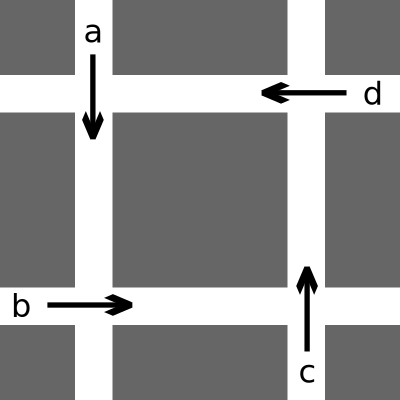
\includegraphics[width=6cm]{img/rightOfWay}
	\caption{Vorfahrt ist nicht transitiv: d hat Vorfahrt vor c hat Vorfahrt vor b hat Vorfahrt vor a hat Vorfahrt vor d}
	\label{fig:rightOfWayNotTransitive}
\end{figure}

Ein Problem beim Überschreiben ist jedoch, dass 'Stummel' vorheriger Markierungen übrig bleiben können, wie in Abb. \ref{fig:overwritingCanCauseStubs} exemplarisch dargestellt. Daher müssen, wenn eine Markierung eines Fahrzeugs entfernt wird, alle Markierungen des Fahrzeugs entfernt werden. Später sind dann die Markierungen des Fahrzeuges neu zu bestimmen.
\begin{figure}[h!]
	\centering
	\includegraphics[width=8cm]{img/stubs}
	\caption{Möglichkeit von Stummeln: Links: A markiert zunächst 4 Felder. Dann rechts: B hat vorfahrt, markiert dabei 3 Felder und überschreibt Markierungen von A. Übberreste der Markierungen von A behindern nun C, der eigentlich fahren könnte}
	\label{fig:overwritingCanCauseStubs}
\end{figure}

Zuletzt muss noch die Anforderung des Einhaltens von Geschwindigkeitsbegrenzungen erfüllt werden. Dazu wird jede Zelle mit einer Maximalgeschwindigkeit versehen. Betritt ein Fahrzeug eine Zelle, wird die maximale Anzahl an Zellen, die es darüber hinaus noch markieren kann auf die Maximalgeschwindigkeit der Zelle gedeckelt. Somit ist gewährleistet, dass kein Fahrzeug an keiner Zelle die zulässige Geschwindigkeit überschreitet.

Diese Überlegungen führen zu folgendem Markierungsalgorithmus:
\lstinputlisting{src/streetMapMarkAlgorithm}
wobei r die verbleibenden Schritte des Autos runterzählt. Ob ein Fahrzeug an einer Zusammenführung Vorfahrt hat, ergibt sich wie oben beschrieben aus der Reihenfolge der Vorgängerverweise. Um die Implementierung zu vereinfachen beschränken wir uns auf Zusammenführungen mit zwei Vorgängern.

Nachdem die Markierungen entsprechend gesetzt wurden müssen im Anschluss daran aus ihnen die tatsächlichen Fahrdistanzen für die einzelnen Fahrzeuge berechnet werden. Dazu kann man in jedem Fahrzeug starten und seine Wunschstrecke solange ablaufen, wie man dabei nur vom Fahrzeug markierte Zellen betritt. Hierbei zählt man eine Variable hoch, die am Ende die Geschwindigkeit des Fahrzeuges angibt. Dies geschieht folgendermaßen:
\lstinputlisting{src/streetMapDistAlgorithm}

Damit haben wir einen Algorithmus erreicht, der beliebige Verkehrsnetze kollisionsfrei unter Berücksichtigung von Vorfahrtsregeln und Geschwindigkeitsbegrenzungen simulieren kann. Im Kontrast zur mehrspurigen Simulation oben kann dieses Verfahren zwar ebenfalls mit mehreren Spuren umgehen, das Rechtsfahrgebot und das Rechtsüberholverbot müssten aber separat implementiert werden. Bis auf das modifizierte Verfahren zur Bestimmung der maximalen Fahrdistanz können die Regeln des Nagel-Schreckenberg Modells \cite{nagel-schreckenberg} übernommen werden. Es werden also zunächst alle Fahrzeuge beschleunigt, dann die Distanzen wie oben beschrieben geprüft, anschließend getrödelt und am Ende die Fahrzeuge bewegt.

Eine schöne Eigenschaft dieser Herangehensweise ist, dass wir ohne zusätzlichen Aufwand Quellen und Senken von Fahrzeugen erzeugen können. Als Quelle wird schlicht jede Zelle definiert, die zwar Nachfolger, aber keine Vorgänger hat. Analog ist jede Zelle eine Senke, die Vorgänger, aber keine Nachfolger hat. Jeder Zelle kann darüber hinaus eine Autoerzeugungswahrscheinlichkeit zugeordnet werden, mit der in der Zelle pro Simulationsschritt ein neues Auto entsteht, sofern sie leer ist. Ein Auto, was eine Senke überfährt, wird hingegen entfernt.

Nun bleibt noch die Frage zu klären, wie an einer Verzweigung die Entscheidung zu treffen ist, in welche Richtung ein Fahrzeug fahren soll (vgl. Zeile 7). Konzeptionell wäre es möglich, jedem neu hinzugefügten Fahrzeug ein Ziel zuzuweisen und einen (randomisierten) Pfadfindungsalgorithmus zu nutzen, um die Entscheidungen an Verzweigungen zu treffen. Da Fahrzeuge in der Regel ein festes Ziel haben, wäre dies der realistischste Ansatz. Zur Vereinfachung der Implementierung entscheiden wir uns allerdings dafür, die Entscheidung an jeder Verzweigung zufällig zu treffen, wobei für jede Nachfolgerzelle individuelle Wahrscheinlichkeiten festgelegt werden können. Da wir nur sehr einfache Straßennetze mit wenigen Verzweigungen (die insbesondere nicht verschachtelt sind) betrachten, erachten wir das als eine ausreichend gute Annäherung. Für komplexere Szenarien werden allerdings komplexere Entscheidungssysteme notwendig.

%TODO: Problem: wenn wir markierungen überschreiben, können 'Stummel' überbleiben, die andere Fahrzeuge blockieren. Illustrieren

\subsection{Visualisierung}
\label{subsec:visualisierung}

\newpage
\section{Ergebnisse}
\label{sec:ergebnisse}
\subsection{Einspurige Straße}
\subsection{Mehrspurige Straße}
\subsection{Kreisverkehr}
Bei der Simulation des Verkehrsflusses an einem Kresverkehr gibt es Verzweigungen und Zusammenführungen, wobei Vorfahrtsregeln und Geschwindigkeitsbegrenzungen zu beachten sind. Daher wird das in Abschnitt \ref{subsec:umsetzung-kreisverkehr} entwickelte Verfahren benutzt. Simuliert wird ein Kreisverkehr mit \texttt{8 Zellen Breite} und \texttt{6 Zellen Höhe}, es handelt sich also näherungsweise um ein Rechteck mit \texttt{60m} Breite und \texttt{45m} Höhe, da wir weiterhin von einer Zellenlänge von $7.5m$ ausgehen. Zum Kreisverkehr führen \texttt{3 Zubringerstraßen bzw. Ausfahrten} die von links, rechts und unten kommen, dementsprechend gibt es \texttt{3 Quellen} und \texttt{3 Senken}. An der Oberseite befinden sich keine Abzweigungen, der Kreisverkehr weist also eine Asymmetrie auf. Die Länge der Zu- und Abfahrten kann variiert werden. Wir entschließen uns dazu, sie auf \texttt{20 Zellen} zu setzen. Zusätzlich gilt die Forderung, dass Fahrzeuge nur mit einer Geschwindigkeit von \texttt{einer Zelle pro Sekunde} in den Kreisverkehr einfahren dürfen, was einer Realgeschwindigkeit von $27km/h$ entspricht. Aufgrund der Proportionen des Kreisverkehrs erscheint es uns auch angemessen, die Geschwindigkeit innerhalb des Kreisverkehrs auf diesen Wert zu beschränken. Da wir von einer Landstraße ausgehen setzen wir das Limit für die Zu- und Abfahrten auf \texttt{4 Zellen/Sekunde}, was $108km/h$ entspricht. Damit ergibt sich die in Abbildung \ref{fig:roundaboutSmall} zu sehenden schematische Darstellung der Straßenkarte.

\begin{figure}[h!]
	\centering
	\includegraphics[width=8cm]{img/roundaboutSmall}
	\caption{Kreisverkehr mit eingetragenen Höchstgeschwindigkeiten}
	\label{fig:roundaboutSmall}
\end{figure}

Schließlich müssen wir noch die Wahrscheinlichkeit, den Kreisverkehr an jeder der Verzweigungen zu verlassen, definieren. Diese wird auf \texttt{1/3} gesetzt, was dazu führt, dass die Wahrscheinlichkeit, die erste oder die zweite Ausfahrt zu nehmen näherungsweise gleich ist, bei der dritten Ausfahrt (wo das Fahrzeug hergekommen ist) aber signifikant geringer.

Mit diesen Parametern lässt sich beobachten, dass sich ab einer \texttt{car generation rate von etwa 1/4} Rückstaus auf dem Zufahrten bilden. Die car generation rate ist dabei die Wahrscheinlichkeit, mit der an jeder der Quellen unabhängig voneinander ein Fahrzeug hinzugefügt wird. Da wir 3 Quellen haben bedeutet dies, dass in jedem Simulationsschritt im Schnitt $3/4$ Autos den Simulationsbereich betreten. Für niedrigere Werte bilden sich keine Rückstaus, für höhere sind sie nahezu garantiert.

Dazu wollen wir uns exemplarisch die Ergebnisse für eine Erzeugungsrate von $0.15$ ansehen, wobei in jeder Runde in etwa $3 \cdot 0.15 = 0.45$ Fahrzeuge die Simulation betreten, also etwa ein Auto in jedem zweiten Simulationsschritt. Abbildung \ref{fig:roundabout015} zeigt einen typischen Zustand des Kreisverkehrs nach 500 Iterationen.

\begin{figure}[h!]
	\centering
	\includegraphics[width=\textwidth]{img/roundabout_015}
	\caption{Erzeugungsrate 0.15. Links: Kreisverkehr nach 500 Iterationen, Mitte: Belegungshäufigkeit, Rechts: Durchschnittsgeschwindigkeit}
	\label{fig:roundabout015}
\end{figure}

Man kann beobachten, dass im Kreisverkehr selbst die Dichte etwas höher ist als an den Auf- und Abfahrten, es ist aber noch genügend Platz für ankommende Autos, die ebenfalls in den Kreisverkehr wollen. Im mittleren Bild sieht man die Belegungshäufigkeit der einzelnen Zellen, und es wird deutlich dass der Kreisverkehr die am intensivsten genutzte Region ist. Dies ist naheliegend, da alle Fahrzeuge diese Region passieren müssen, jede Zufahrtsstraße aber nur von einem Drittel der Autos genutzt wird. Die Durchschnittsgeschwindigkeit in jeder Zelle lässt sich dem rechten Bildteil entnehmen, wobei man sieht dass auf den Zufahrtsstraßen die Durchschnittsgeschwindigkeit der Maximalgeschwindigkeit 4 entspricht. Vom Kreisverkehr bzw. den Quellen weg wird auf diesen Wert beschleunigt. Bei der Anfahrt auf den Kreisverkehr kann es zuweilen vorkommen, dass man auf eine Einfahrmöglichkeit warten muss, weswegen sich die Geschwindigkeit graduell verlangsamt je näher man kommt.

Das Verhalten des Systems über die Zeit zeigt die Abbildung \ref{fig:roundabout015density}, in der die Verkehrsdichte gegen die Zeit in Simulationsschritten abgetragen ist. Sie ist deutlichen Schwankungen unterworfen, die sich aus dem Herausfahren von Fahrzeugen und dem zufälligen Neuerzeugen ergeben. Sie bleibt aber etwa mit 0.14 nach oben beschränkt, was zeigt dass der Verkehr flüssig fahren kann.

\begin{figure}[h!]
	\centering
	\includegraphics[width=\textwidth]{img/roundabout_015_densities}
	\caption{Dichte im Kreisverkehr über 500 iterationen bei Erzeugungsrate 0.15}
	\label{fig:roundabout015density}
\end{figure}

Erhöhen wir die Erzeugungsrate auf 0.35, so zeigt sich ein anderes Bild. Es betreten nun in jedem Simulationsschritt im Mittel etwa $3 \cdot 0.35 = 1.05$ Fahrzeuge, also etwas mehr als eines, die Simulation. Die dazugehörigen Messwertbilder sind in Abbildung \ref{fig:roundabout035} zu sehen und unterscheiden sich deutlich von denen für eine Erzeugungsrate von 0.15.

\begin{figure}[h!]
	\centering
	\includegraphics[width=\textwidth]{img/roundabout_035}
	\caption{Erzeugungsrate 0.35. Links: Kreisverkehr nach 500 Iterationen, Mitte: Belegungshäufigkeit, Rechts: Durchschnittsgeschwindigkeit}
	\label{fig:roundabout035}
\end{figure}

Zunächst fällt auf dass der Kreisverkehr komplett gefüllt ist. Da sich die Fahrzeuge im Kreis alle mit Geschwindigkeit 1 bewegen und Vorfahrt haben sind in jeder Runde alle Felder belegt. Da auf den Zufahrtsstraßen aber weiterhin Fahrzeuge ankommen bildet sich hier ein Rückstau, der Stellenweise Lücken aufweist wo Autos einem in den Kreis eingefahrenen nachrücken. Dies zeigt sich auch an der Belegungshäufigkeit der Zellen, die auf den Zufahrtsstraßen nun wesentlich höhere Werte annimmt. Wo vormals eine in etwa gleiche Nutzung von Zu- und Abfahrtsstraßen zu sehen war tritt nun eine starke Diskrepanz auf, wobei die Auslastung im Kreisverkehr weiterhin hoch ist. Die Durchschnittsgeschwindigkeiten sind dementsprechend geringer. Wärend innerhalb des Kreisverkehrs aufgrund der Vorfahrt eine Zelle vor jedem Fahrzeug frei bleibt und des dementsprechend nicht zu systematischen Staus kommt stehen die Fahrzeuge auf den Zufahrtsstraßen über weite Teile der Strecke und müssen warten, bis der Vorderste in den Kreisverkehr einfahren kann. Fahrzeuge, die die Abfahrtsstraßen erreichen können ungehindert beschleunigen, da sie in der Regel keine Autos vor sich haben.

\begin{figure}[h!]
	\centering
	\includegraphics[width=\textwidth]{img/roundabout_035_densities}
	\caption{Dichte im Kreisverkehr über 500 iterationen bei Erzeugungsrate 0.35}
	\label{fig:roundabout035density}
\end{figure}

Der Verlauf der Verkehrsdichte zu diesem Durchlauf ist in Abbildung \ref{fig:roundabout035density} dargestellt. Zu Beginn der Simulation befinden sich nur wenige Fahrzeuge auf der Strecke, dieser Wert steigt allerdings durch die ankommenden Fahrzeuge kontinuierlich, bis er sich um eine Dichte von etwa $0.4$ einpendelt. Dies entspicht dem Zeitpunkt, ab dem aus Platzgründen keine Fahrzeuge mehr an den Quellen generiert werden können bis ein Fahrzeug den Kreisverkehr verlässt und andere nachrücken können.

\subsection{Autobahnkreuz}

\newpage
\section{Fazit}
\label{sec:fazit}

%\blindtext asdf \cite{mehrspurig}\\
%In Kapitel \myref{sec:einleitung} steht Shit. In Foobar (\myrefcomma{sec:ansatz}) bla

\newpage
\addcontentsline{toc}{section}{Literatur}
\bibliography{ref}{}
\bibliographystyle{alpha}

\end{document}